%%%%%%%%%%%%%%%%%%%%%%%%%%%%%%%%%%%%%%%%%%%%%%%%%%%%%%%%%%%%%%%%%%%%%%
% LaTeX Template: Beamer arrows
%
% Source: http://www.texample.net/
% Feel free to distribute this template, but please keep the
% referal to TeXample.net.
% Date: Nov 2006
% 
%%%%%%%%%%%%%%%%%%%%%%%%%%%%%%%%%%%%%%%%%%%%%%%%%%%%%%%%%%%%%%%%%%%%%%
% How to use writeLaTeX: 
%
% You edit the source code here on the left, and the preview on the
% right shows you the result within a few seconds.
%
% Bookmark this page and share the URL with your co-authors. They can
% edit at the same time!
%
% You can upload figures, bibliographies, custom classes and
% styles using the files menu.
%
% If you're new to LaTeX, the wikibook is a great place to start:
% http://en.wikibooks.org/wiki/LaTeX
%
%%%%%%%%%%%%%%%%%%%%%%%%%%%%%%%%%%%%%%%%%%%%%%%%%%%%%%%%%%%%%%%%%%%%%%

\documentclass[handout]{beamer} %
\usetheme{CambridgeUS}
\usepackage[latin1]{inputenc}
\usefonttheme{professionalfonts}
\usepackage{times}
\usepackage{tikz}
\usepackage{amsmath}
\usepackage{verbatim}
\usetikzlibrary{arrows,shapes}
\beamertemplatenavigationsymbolsempty

\AtBeginSection[]{
\frame{\frametitle{}
\tableofcontents[current]}
}

\author[]{Shao Group Meeting}
\institute[]{University of Oklahoma }
\title[]{Hartree-Fock Theory}
\date[September 2017]{September 2017}

\begin{document}

\begin{comment}
:Title: Beamer arrows
:Tags: Remember picture, Beamer, Physics & chemistry, Overlays
:Use page: 3

With PGF/TikZ version 1.09 and later, it is possible to draw paths between nodes across
different pictures. This is a useful feature for presentations with the
Beamer package. In this example I've combined the new PGF/TikZ's overlay feature
with Beamer overlays. Download the PDF version to see the result.
**Note.** This only works with PDFTeX, and you have to run PDFTeX twice.
| Author: Kjell Magne Fauske

\end{comment}


% For every picture that defines or uses external nodes, you'll have to
% apply the 'remember picture' style. To avoid some typing, we'll apply
% the style to all pictures.
\tikzstyle{every picture}+=[remember picture]

% By default all math in TikZ nodes are set in inline mode. Change this to
% displaystyle so that we don't get small fractions.
\everymath{\displaystyle}

\frame{\titlepage}

\begin{frame}
\frametitle{Schr\"{o}dinger equation for a molecular system}

\begin{itemize}
\item \small{The Schr\"{o}dinger equation is}
\begin{equation*}
\hat{H} \Psi(\vec{r}_1, \vec{r}_2, \cdots, \vec{r}_N)  = E \Psi(\vec{r}_1, \vec{r}_2, \cdots, \vec{r}_N)  
\end{equation*}
\item The Hamiltonian is
\begin{eqnarray*}
\hat{H} & = &  \sum_i \left(- \frac{1}{2} \bigtriangledown_i^2  - \sum_A \frac{Z_A}{\left| \vec{r}_i - \vec{R}_A \right| } \right) +  \sum_{i < j} \frac{1}{\left| \vec{r}_{i} - \vec{r}_j \right| }   \end{eqnarray*}
\end{itemize}
which includes 
\begin{itemize}
\item \small{kinetic energy, $- \frac{1}{2} \bigtriangledown_i^2$, of each electron}
\item nuclear attraction $- \sum_A \frac{Z_A}{\left| \vec{r}_i - \vec{R}_A \right| } $
\item electron-electron repulsion, $ \sum_{i < j} \frac{1}{\left| \vec{r}_{i} - \vec{r}_j \right| } $ 
\end{itemize}
\end{frame}

\begin{frame}
\frametitle{Hartree-Fock wavefunction: Slater determinants}
\begin{itemize} \itemsep 1mm
\item  \small{For $N$ electrons in $N$ molecular orbitals, the Slater determinant is }
\footnotesize{
\begin{eqnarray*}
\Psi(\vec{r}_1, \vec{r}_2, \cdots, \vec{r}_N)  = \frac{1}{\sqrt{(N)!}} 
\begin{vmatrix} 
   \psi_{1} (\vec{r}_1)  &  \psi_{2} (\vec{r}_1)  & \cdots &    \psi_{N} (\vec{r}_1) \\
  \psi_{1} (\vec{r}_2)  &  \psi_{2} (\vec{r}_2)  & \cdots &    \psi_{N} (\vec{r}_2) \\
   \cdots & \cdots & \cdots & \cdots \\   
   \psi_{1} (\vec{r}_N)  &  \psi_{2} (\vec{r}_N)  & \cdots &    \psi_{N} (\vec{r}_N)
\end{vmatrix} 
\end{eqnarray*}  
}  
\item Each molecular orbital is a linear combination of basis functions
\begin{equation*}
\psi_i(\vec{r}) = \sum_{\mu} C_{\mu i} \phi_{\mu} ({\vec{r}}) 
\end{equation*} 
\item In most quantum chemistry calculations, we use Gaussian functions
\begin{equation*}
\phi_{\mu} ( \mathbf{a}; \vec{r}) = (x-A_x)^{a_x} (y-A_y)^{a_y} (z-A_z)^{a_z} \sum_k D_k exp\left(-\alpha_k |\vec{r} - \vec{A} | ^2 \right) 
\end{equation*}
with $\alpha_k$ are called exponents, and $D_k$ contraction coefficients. 
\item Plane-wave basis functions can be used in QM calns on solid/surface systems. 
\end{itemize}
\end{frame}

\begin{frame}
\frametitle{Why Gaussian Basis Sets?}
\begin{itemize}
\item Gaussian Product Theorem for 1-D Functions
\begin{eqnarray*}
e^{-\alpha (x-A_x)^2} e ^{-\beta (x-B_x)^2}  & = & e^{ -(\alpha+\beta)x^2 + 2 (\alpha A_x +  \beta B_x) x - (\alpha A_x^2 + \beta B_x^2)  }   \\
& = & e^{- (\alpha+\beta) ( x - \frac{\alpha A_x +  \beta B_x} { \alpha + \beta} )^2 + \frac{(\alpha A_x +  \beta B_x)^2}{\alpha + \beta}  - (\alpha A_x^2 + \beta B_x^2)  } \\
& = &  e^{- (\alpha+\beta) ( x - \frac{\alpha A_x +  \beta B_x} { \alpha + \beta} )^2  - \frac{ \alpha \beta} { \alpha + \beta} ( A_x-B_x) ^2 } 
\end{eqnarray*}
\visible<2->{
\item Gaussian Product Theorem for 3-D Functions
\footnotesize{
\begin{eqnarray*}
e^{-\alpha (r-A)^2} e ^{-\beta (r-B)^2}  & = & e^{-\alpha \left[ (x-A_x)^2 + (y-A_y)^2 + (z-A_z)^2 \right] }   \\
  & & \times e^{- \beta \left[ (x-B_x)^2 + (y-B_y)^2 + (z-B_z)^2\right] }   \\
  & = & e^{- (\alpha + \beta) \left[ (x-P_x)^2 + (y-P_y)^2 + (z-P_z)^2 \right]  }  \\
  &  & \times e^{  - \frac{ \alpha \beta} { \alpha + \beta} \left[ ( A_x-B_x) ^2 + (A_y-B_y)^2 + (A_z-B_z)^2 \right] }  \\
  & = & e^{ - (\alpha + \beta)  \left| \vec{r} - \vec{P} \right|^2 } e^{-  \frac{ \alpha \beta} { \alpha + \beta}  \left| \vec{A}-\vec{B} \right|^2 } 
\end{eqnarray*}
}
where $\vec{P} = \frac{ \alpha \vec{A} + \beta \vec{B}} {\alpha + \beta}$.  }\visible<3->{   This means that we can convert 4-center 2-electron integrals $(a b | c d)$ into 2-center 2-electron integrals $(p|q)$.  }

\end{itemize}
\end{frame}

\begin{frame}
\frametitle{6-31G Basis Functions for Helium Atom}
\begin{columns}
\begin{column}{0.5\textwidth}
\begin{itemize}
\item The basis set specification is 
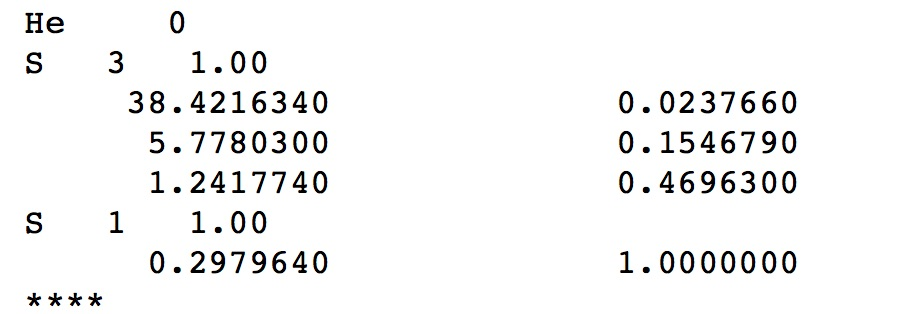
\includegraphics[height=0.8in]{figures/gaussian-he2.jpg}
\vspace{3mm}
\visible<2->{
\item 1st function has 3 Gaussians
\scriptsize{
\begin{eqnarray*}
\phi_1 & = &  N_t ( 0.023766 * N_1 *e^{-38.421634 r^2} \\ 
& & + 0.154679  * N_2 * e^{-5.77803 r^2} \\
& & + 0.46963 * N_3 * e^{-1.241774 r^2} ) 
\end{eqnarray*}
}
}
\vspace{-4mm}
\visible<3->{
\item \small{2nd function has 1 Gaussian}
\scriptsize{
\begin{equation*}
\phi_2 = N_4 e^{-0.2927640 r^2} 
\end{equation*}
}
}
\end{itemize}
\end{column}
\begin{column}{0.5\textwidth}
\vspace{-3mm}
\visible<4->{
\begin{center}
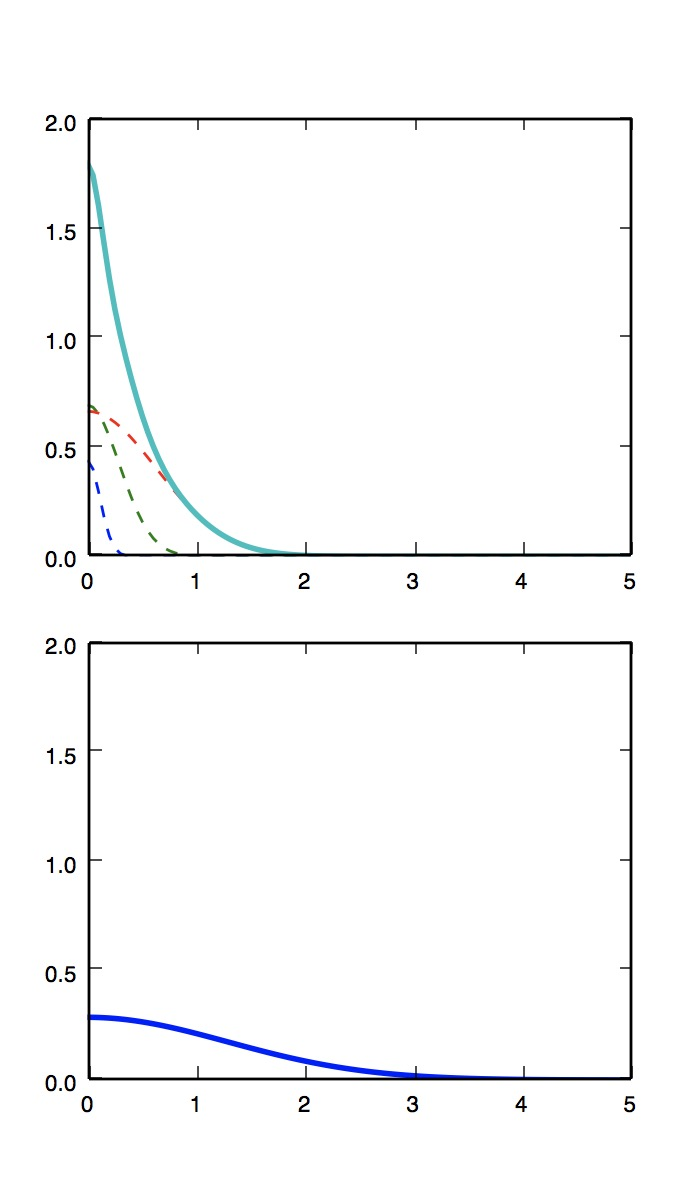
\includegraphics[height=3.2in]{figures/gaussian-he.jpg}
\end{center}
}
\end{column}
\end{columns}
\end{frame}

\begin{frame}
\frametitle{Pople Gaussian Basis Sets}
\scriptsize{
\begin{table}
\begin{tabular}{lcccc}
\hline \hline 
basis &  & H, He & Li, Be, B, C, N, O, F, Ne & Comment \\
\hline \\
STO-3G & core & &  3s $\rightarrow$ 1s & Too small   \\
    & valence & 3s $\rightarrow$ 1s & 3s3p $\rightarrow$ 1s1p &   \\  \\
\textcolor{red}{6}-\textcolor{blue}{31}G\textcolor{purple}{*} & core &  &   \textcolor{red}{6s  $\rightarrow$ 1s } & \\  
  & valence & \textcolor{blue}{4s  $\rightarrow$ 2s} & \textcolor{blue}{4s4p}\textcolor{purple}{1d}  $\rightarrow$ \textcolor{blue}{2s2p}\textcolor{purple}{1d} & \\  \\
\textcolor{red}{6}-31++G\textcolor{purple}{*}\textcolor{green}{*} & core & & \textcolor{red}{6s  $\rightarrow$ 1s} &  medium \\  
  & valence & 5s\textcolor{green}{1p}  $\rightarrow$ 3s\textcolor{green}{1p} & 5s5p\textcolor{purple}{1d}  $\rightarrow$ 3s3p\textcolor{purple}{1d} \\ \\
\textcolor{red}{6}-311++G\textcolor{purple}{*}\textcolor{green}{*} & core & & \textcolor{red}{6s  $\rightarrow$ 1s} &  large \\  
  & valence & 6s\textcolor{green}{1p}  $\rightarrow$ 4s\textcolor{green}{1p} & 6s6p\textcolor{purple}{1d}  $\rightarrow$ 4s4p\textcolor{purple}{1d} \\  \\
  \textcolor{red}{6}-311++G(3df,3pd) & core & & \textcolor{red}{6s  $\rightarrow$ 1s} &  largest \\
  & valence & 6s3p1d  $\rightarrow$ 4s3p1d & 6s6p3d1f $\rightarrow$ 4s4p3d1f \\ \\

\hline \hline
\end{tabular}
\end{table}
}
\begin{itemize}
\item See https://bse.pnl.gov/bse/portal for details
\visible<2->{
\item Dunning basis set (cc-pVDZ, aug-cc-pVDZ, cc-pVTZ, aug-cc-pVTZ, cc-pVQZ, aug-cc-pVQZ) are equally (if not more) popular}
\end{itemize}

\end{frame}

\begin{frame}
\frametitle{Hartree-Fock Energy for a Slater Determinant}

\begin{itemize}

\item  \small{For $N$ electrons in $N$ molecular orbitals, the Slater determinant is }
\footnotesize{
\begin{eqnarray*}
\Psi(\vec{r}_1, \vec{r}_2, \cdots, \vec{r}_N)  = \frac{1}{\sqrt{(N)!}} 
\begin{vmatrix} 
   \psi_{1} (\vec{r}_1)  &  \psi_{2} (\vec{r}_1)  & \cdots &    \psi_{N} (\vec{r}_1) \\
  \psi_{1} (\vec{r}_2)  &  \psi_{2} (\vec{r}_2)  & \cdots &    \psi_{N} (\vec{r}_2) \\
   \cdots & \cdots & \cdots & \cdots \\   
   \psi_{1} (\vec{r}_N)  &  \psi_{2} (\vec{r}_N)  & \cdots &    \psi_{N} (\vec{r}_N)
\end{vmatrix} 
\end{eqnarray*}  
}  
The energy of this Slater determinant is 
\begin{equation*}
E_{HF} = \sum_{i=1}^N h_i + \sum_{i<j}^{N} \left[ (ii|jj) - (ij|ij) \right]
\end{equation*}
where 
\scriptsize{
\begin{eqnarray*}
h_{i} & = & \int d\vec{r}~ \psi^*_i (\vec{r}) \left[ -\frac{1}{2} \bigtriangledown^2 - \sum_A \frac{Z_A}{ \left| \vec{r} - \vec{R}_A \right| } \right] \psi_i (\vec{r})  \\
(ii|jj) &  =  & \iint d\vec{r}_1 d\vec{r}_2 \psi^*_i (\vec{r}_1) \psi^*_i(\vec{r}_1) \frac{1}{r_{12}} \psi_j ( \vec{r}_2)  \psi_j(\vec{r}_2)   \\
(ij|ij) &  =  & \iint d\vec{r}_1 d\vec{r}_2 \psi^*_i (\vec{r}_1) \psi^*_{\textcolor{red}{j}}(\vec{r}_1) \frac{1}{r_{12}} \psi_{\textcolor{red}{i}} (\vec{r}_2)  \psi_j(\vec{r}_2)  
\end{eqnarray*}
}
\end{itemize}
\end{frame}

\begin{frame}
\begin{itemize}
\item \small{Hartree-Fock energy (of a Slater determinant) is }
\begin{eqnarray*}
E_{HF} & = & \sum_{i=1}^N h_i + \sum_{i<j}^{N} \left[ (ii|jj) - (ij|ij) \right]   \\
& = & \sum_{i=1}^N h_i + \frac{1}{2} \sum_{i=1}^N \sum_{j=1}^{N} \left[ (ii|jj) - (ij|ij) \right]   
\end{eqnarray*}
\item We search for an optimal set of occupied molecule orbitals, $\psi_i(\vec{r})$, to minimize this energy.   In practice, this is done through the self-consistent field (SCF) procedure. 
\item In DFT calculations, the $i=j$ term of Coulomb energy is no longer cancelled by its Hartree Fock exchange counterpart.   This is called the self-interaction error.   
\end{itemize}
\end{frame}

\begin{frame}
\frametitle{Electron Density and Density Matrix} 
\begin{itemize}
\item \footnotesize{Given a set of \textcolor{red}{orthonormal} occupied molecular orbitals, $\psi_i(\vec{r})$, we can write the electron density as }
\begin{eqnarray*}
\rho(\vec{r}) & =  & \sum_{i=1}^N (\psi_i(\vec{r})) ^2  \\
& = & \sum_{i=1}^N  \left[ \sum_{\mu} C_{\mu i} \phi_{\mu}(\vec{r}) \right]   \left[ \sum_{\nu} C_{\nu i} \phi_{\nu}(\vec{r}) \right]  \\
& = & \sum_{\mu, \nu}  \left[ \sum_i   C_{\mu i}  C_{\nu i}\right]    \phi_{\mu}(\vec{r})  \phi_{\nu}(\vec{r})  \\
& = & \sum_{\mu, \nu}  P^{\mu \nu}     \phi_{\mu}(\vec{r})  \phi_{\nu}(\vec{r})  
\end{eqnarray*}
\item (One-Particle) Density matrix is 
\begin{equation*}
 P^{\mu \nu} =  \sum_i   C_{\mu i}  C_{\nu i}      ~~~~~~~ P = C_o C_o ^{\dagger} 
\end{equation*}
\end{itemize}
\end{frame}

\begin{frame}
\frametitle{Hartree-Fock Energy in AO Representation} 
\begin{itemize}
\item \footnotesize{The Hartree-Fock energy}
\begin{equation*}
E_{HF} = \sum_{i=1}^N h_i + \frac{1}{2} \sum_{i=1}^N \sum_{j=1}^{N} \left[ (ii|jj) - (ij|ij) \right]
\end{equation*}
\item can be rewritten as
\begin{equation*}
E_{HF} =  \sum_{\mu \nu}   P^{\mu \nu}  h_{\mu\nu} + \frac{1}{2} \sum_{\mu \nu, \lambda \sigma} P^{\mu \nu}  ( \mu \nu | \lambda \sigma ) P^{\lambda \sigma}   
- \frac{1}{2} \sum_{\mu \nu, \lambda \sigma} P^{\mu \nu}  ( \mu \lambda | \nu \sigma ) P^{\lambda \sigma}  
\end{equation*}
This is the Hartree-Fock energy expression in the atomic orbital (AO) representation. 
\item This requires one-electron and two-electron integrals
\begin{eqnarray*}
h_{\mu \nu} & = &  \int d\vec{r}~ \phi_{\mu} (\vec{r}) \left[ -\frac{1}{2} \bigtriangledown^2 - \sum_A \frac{Z_A}{ \left| \vec{r} - \vec{R}_A \right| } \right] \phi_{\nu} (\vec{r})    \\
( \mu \nu | \lambda \sigma )  & = &  ~~~ \int \int d\vec{r_1}  d\vec{r_2}    \phi_{\mu} (\vec{r})  \phi_{\nu} (\vec{r})  \frac{1}{r_{12}}    \phi_{\lambda} (\vec{r})  \phi_{\sigma} (\vec{r}) 
\end{eqnarray*} 

\end{itemize}
\end{frame}

\begin{frame}
\frametitle{Concise Notation for Hartree-Fock Energy}
\begin{itemize}
\item \footnotesize{Hartree-Fock energy is}
\begin{eqnarray*}
E_{HF} & = &  \sum_{\mu \nu}   P^{\mu \nu}  h_{\mu\nu} + \frac{1}{2} \sum_{\mu \nu, \lambda \sigma} P^{\mu \nu}  ( \mu \nu | \lambda \sigma ) P^{\lambda \sigma}   
- \frac{1}{2} \sum_{\mu \nu, \lambda \sigma} P^{\mu \nu}  ( \mu \lambda | \nu \sigma ) P^{\lambda \sigma}   \\
& = &  \sum_{\mu \nu}   P^{\mu \nu}  h_{\mu\nu} + \frac{1}{2} \sum_{\mu \nu, \lambda \sigma} P^{\mu \nu}  \left[ ( \mu \nu | \lambda \sigma ) -  ( \mu \lambda | \nu \sigma ) \right] P^{\lambda \sigma}  \\
& = & \sum_{\mu \nu}   P^{\mu \nu}  h_{\mu\nu} + \frac{1}{2} \sum_{\mu \nu, \lambda \sigma} P^{\mu \nu} ( \mu \nu \textcolor{red}{||} \lambda \sigma ) P^{\lambda \sigma}   \\
& = & P \cdot h + \frac{1}{2} P \cdot \Pi \cdot P 
\end{eqnarray*}
where
\begin{eqnarray*}
\Pi_{\mu \nu, \lambda \sigma} =  ( \mu \nu \textcolor{red}{||} \lambda \sigma )  = ( \mu \nu | \lambda \sigma ) -  ( \mu \lambda | \nu \sigma ) 
\end{eqnarray*} 
\end{itemize}
\end{frame}

\begin{frame}
\frametitle{\normalsize Fock Matrix}
\vspace{-3mm}
\begin{itemize}
\item \footnotesize{The general definition of Fock matrix (for both Hartree-Fock and DFT) is}
\begin{equation*}
F_{\mu \nu} = \frac {\partial  E} {\partial P^{\mu \nu}}   
\end{equation*}
which will be shown to be equal to be $ ( \phi_{\mu} |  \hat{f} | \phi_{\nu} )$, namely an AO representation of the Fock operator (one-electron effective Hamiltonian).   
\item From the energy expression, 
\begin{eqnarray*}
E_{HF} =  \sum_{\mu \nu}   P^{\mu \nu}  h_{\mu\nu} + \frac{1}{2} \sum_{\mu \nu, \lambda \sigma} P^{\mu \nu} ( \mu \nu \textcolor{red}{||} \lambda \sigma ) P^{\lambda \sigma} 
\end{eqnarray*}
we can derive
\begin{eqnarray*}
F_{\mu \nu} = \frac {\partial  E} {\partial P^{\mu \nu}}    & = &   h_{\mu \nu} + \sum_{ \lambda \sigma} ( \mu \nu \textcolor{red}{||} \lambda \sigma ) P^{\lambda \sigma}   \\
& = & h_{\mu \nu} + \sum_{ \lambda \sigma} ( \mu \nu | \lambda \sigma ) P^{\lambda \sigma}   -  \sum_{ \lambda \sigma} ( \mu \lambda | \nu \sigma ) P^{\lambda \sigma}  \\
& = &  h_{\mu \nu}  +  J_{\mu \nu}  - K_{\mu \nu}   
\end{eqnarray*} 
where $J_{\mu \nu}$ is the Coulomb matrix, and $K_{\mu \nu}$ the exchange matrix.  
\item In concise notation, 
\begin{eqnarray*}
F = h + \Pi \cdot P = h + J - K 
\end{eqnarray*} 
\end{itemize}
\end{frame}

\end{document}

\begin{frame}
\begin{itemize}
\item \textcolor{blue}{Quiz:}  The 2-electron exchange integral is
\begin{equation*}
(ij|ij)  =  \iint d\tau_1 d\tau_2 \psi^*_i (\tau_1) \psi^*_{\textcolor{red}{j}}(\tau_1) \frac{1}{r_{12}} \psi_{\textcolor{red}{i}} (\tau_2)  \psi_j(\tau_2)  
\end{equation*} 
What is its value, if the two spin orbitals $\psi_i$ and $\psi_j$ have different spin? 
\begin{itemize}
\item Zero
\item Nonzero
\end{itemize}
\end{itemize}
\end{frame}

\section{Hartree-Fock Theory}

\begin{frame}
\begin{itemize}
\item Let us rewrite the energy 
\small{
\begin{eqnarray*}
E_{HF}  & = &  \sum_{i=1}^N h_i +   \sum_{i<j}^{N} \left[ (ii|jj) - (ij|ij) \right]   \\
& = &  \sum_{i=1}^N h_i + \frac{1}{2} \sum_{i \neq j}^{N} \left[ (ii|jj) - (ij|ij) \right]  \\
& = & \sum_{i=1}^N h_i + \frac{1}{2} \sum_{i, j}^{N} \left[ (ii|jj) - (ij|ij) \right] 
\end{eqnarray*}
}
\visible<2->{
\item Add the normalization constraint
\begin{eqnarray*}
\tilde{E} =  \sum_{i=1}^N h_i + \frac{1}{2} \sum_{i, j}^{N} \left[ (ii|jj) - (ij|ij) \right]  \textcolor{red}{- \sum_i \epsilon_i \left[ ( i | i) - 1 \right] }
\end{eqnarray*}
where 
\begin{equation*}
(i | i ) = \int d\tau~ \psi^*_i (\tau) \psi_i (\tau)  
\end{equation*}
}

\end{itemize}
\end{frame}

\begin{frame}
\begin{itemize}
\item Apply the variational principle on 
\begin{eqnarray*}
\tilde{E} =  \sum_{i=1}^N h_i + \frac{1}{2} \sum_{i, j}^{N} \left[ (ii|jj) - (ij|ij) \right]  - \sum_i \epsilon_i \left[ ( i | i)  -1 \right]
\end{eqnarray*}
\item We will find an equation for each spin orbital
\begin{equation*}
\hat{F} ( \tau_1 )  \psi_i (\tau_1) = \epsilon_i \psi_i (\tau_1) 
\end{equation*}
\visible<2->{
where $\hat{F}$ is the Fock operator
\footnotesize{
\begin{equation*}
\hat{F} (\tau_1) = \hat{h} (\tau_1)  + \sum_j^N \left[ \hat{J}_j (\tau_1) - \hat{K}_j (\tau_1) \right] 
\end{equation*}
}
}
\visible<3->{
\small{$\hat{J}$ is the Coulomb operator, $\hat{K}$ is the exchange operator}
\footnotesize{
\begin{eqnarray*} 
\hat{J}_j (\tau_1)  \psi_i (\tau_1) & = &  \left[ \int d\tau_2 \frac{1}{r_{12}} \psi^*_j (\tau_2) \psi_j (\tau_2) \right] \psi_i (\tau_1)   \\ 
\hat{K}_j (\tau_1)  \psi_i (\tau_1) & = &  \left[ \int d\tau_2 \frac{1}{r_{12}} \psi^*_j (\tau_2) \psi_{\textcolor{red}{i}} (\tau_2) \right] \psi_{\textcolor{red}{j}} (\tau_1) 
\end{eqnarray*}
}
}
\end{itemize}
\end{frame}

\begin{frame}
\frametitle{Hartree-Fock Theory}
\begin{itemize}
\item Working equation
\begin{equation}
\hat{F} ( \tau_1 )  \psi_i (\tau_1) = \epsilon_i \psi_i (\tau_1) 
\end{equation}
with
\scriptsize{
\begin{eqnarray*}
\hat{F} (\tau_1) & =  & \hat{h} (\tau_1)  + \sum_j^N \left[ \hat{J}_j (\tau_1) - \hat{K}_j (\tau_1) \right]  \\
\hat{J}_j (\tau_1)  \psi_i (\tau_1) & = &  \left[ \int d\tau_2 \frac{1}{r_{12}} \psi^*_j (\tau_2) \psi_j (\tau_2) \right] \psi_i (\tau_1)   \\ 
\hat{K}_j (\tau_1)  \psi_i (\tau_1) & = &  \left[ \int d\tau_2 \frac{1}{r_{12}} \psi^*_j (\tau_2) \psi_{\textcolor{red}{i}} (\tau_2) \right] \psi_{\textcolor{red}{j}} (\tau_1) 
\end{eqnarray*}
}
\visible<2->{
\item \small{We want to solve Eq.1 (the eigenvalue problem for the Fock operator, $\hat{F}$) to obtain the spin orbitals. }}
\visible<3->{
\item \small{But the Fock operator depends on all spin orbitals.  }}
\visible<3->{
\item In practice, the equation is solved iteratively (i.e. self-consistently).  }
\visible<4->{
\item So the Hartree-Fock theory is also known as the Self-Consistent-Field (SCF) theory.}
\end{itemize}
\end{frame}

\begin{frame}
\frametitle{Basis set}
\begin{itemize}
\item Each atomic orbital is represented as a linear combination of basis functions
\footnotesize{
\begin{equation*}
\psi_i(r) = \sum_{\nu} C_{\nu i} \phi_{\nu} (r) 
\end{equation*} 
}
\visible<2->{
\item \small{The eigen-equation becomes }
\footnotesize{
\begin{equation*}
\hat{F} (r) \left[  \sum_{\nu} C_{\nu i} \phi_{\nu} (r)  \right] = \epsilon_i \sum_{\nu} C_{\nu i} \phi_{\nu} (r)  
\end{equation*}
}
}
\visible<3->{
\item \small{Left multiply by $\phi^*_{\mu} (r)$ and integrate over space,}
\footnotesize{
\begin{eqnarray*}
\sum_{\nu}  \left[  \int dr \phi^*_{\mu} (r) \hat{F} (r)  \phi_{\nu} (r) \right]   C_{\nu i}& = &  \epsilon_i \sum_{\nu}  \left[  \int dr \phi^*_{\mu} (r) \phi_{\nu} (r) \right]   C_{\nu i} \\
 \sum_{\nu} F_{\mu \nu} C_{\nu i}  & = &  \epsilon_i \sum_{\nu}  S_{\mu \nu}   C_{\nu i}    \\
 \mathbf{F~C} & = &  \mathbf{S~ C}~\epsilon
\end{eqnarray*}
} 
}
\end{itemize}
\end{frame}

\begin{frame}
\frametitle{Hartree-Fock-Roothaan Equation}
\begin{itemize}
\item With each atomic orbital as a linear combination, 
\begin{equation*}
\psi_i(r) = \sum_{\nu} C_{\nu i} \phi_{\nu} (r) 
\end{equation*} 
\item The equation to solve is 
\begin{equation*}
\mathbf{FC}  =   \mathbf{S C} ~  \epsilon
\end{equation*}
\visible<2->{
where $\mathbf{F}$ is the Fock matrix, $\mathbf{S}$ is the overlap matrix, 
\begin{eqnarray*}
F_{\mu \nu} & = &   \int dr \phi^*_{\mu} (r) \hat{F} (r)  \phi_{\nu} (r)  \\
S_{\mu \nu} & = &    \int dr \phi^*_{\mu} (r) \phi_{\nu} (r)
\end{eqnarray*}
}

\end{itemize}
\end{frame}

\begin{frame}
\begin{itemize}
\item The Fock matrix
\begin{equation*}
F_{\mu \nu} = h_{\mu \nu} + J_{\mu \nu} - K_{\mu \nu}  
\end{equation*}
\visible<2->{
\item where the three components are
\begin{eqnarray*}
h_{\mu \nu} & = & \int dr_1 \phi^*_{\mu} (r_1) \hat{h}_1 \phi_{\nu}(r_1)  \\
J_{\mu \nu} & = & \sum_i \iint dr_1  dr_2~\phi^*_{\mu} (r_1) \phi_{\nu} (r_1) \frac{1}{r_{12}} \psi^*_i (r_2) \psi_i (r_2)  \\
K_{\mu \nu} & = & \sum_i \iint dr_1  dr_2~\phi^*_{\mu} (r_1) \textcolor{red}{\psi_{i} (r_1)} \frac{1}{r_{12}} \psi^*_i (r_2) \textcolor{red}{\phi_{\nu}(r_2)}   
\end{eqnarray*}
where $J$ is the Coulomb matrix and $K$ is the exchange matrix. 
}
\end{itemize}
\end{frame}

\begin{frame}
\frametitle{Hartree-Fock Solutions for the Helium Atom}
\begin{itemize}
\item \textcolor{blue}{Solution 1:} atomic orbital is approximated as a sum of 2 exponentials
\begin{equation*}
\psi(r) = \sum_{i=1}^2 C_i N_i e^{-\alpha_i r} 
\end{equation*}
where $N_i$ are the normalization coefficients.   \visible<2->{The exponents are: 
\begin{eqnarray*}
\alpha & = &  \{ 1.45363, 2.91093\}  
\end{eqnarray*}
}
\visible<3->{
\item In the self-consistent field (SCF) procedure, we observe
\tiny{
\begin{table}
\begin{tabular}{lcccccccc}
\hline \hline
Iteration & 1 & 2 & 3 & 4 & 5 & 6 & 7 & 8  \\
\hline 
$C_1$ & 0.5 & 0.884622 & 0.835790 & 0.845342 & 0.843481 & 0.843844 & 0.843773 & 0.843787  \\
$C_2$ & 0.5 & 0.134530 & 0.189639 & 0.178940 & 0.181028 & 0.180621 & 0.180700 & 0.180685 \\
$\epsilon$ & -0.89072 & -0.93454 & -0.91472 & -0.91856 & -0.91781 & -0.91796 & -0.91793 & -0.91794 \\
$E$ & -2.490200 & -2.85713 & -2.86150 & -2.86167 &  -2.86167 &  -2.86167 &  -2.86167 &  -2.86167 \\
\hline \hline
\end{tabular}
\end{table}
} 
Note that $S_{12}$ is 0.837.   The spin orbital at the first cycle is not normalized. 
}
\end{itemize}
\end{frame}

\begin{frame}
\frametitle{Hartree-Fock Solutions for the Helium Atom}
\begin{itemize}
\item \textcolor{blue}{Solution 2:} atomic orbital is approximated a sum of 5 exponentials
\begin{equation*}
\psi(r) = \sum_{i=1}^5 C_i N_i e^{-\alpha_i r} 
\end{equation*}
where $N_i$ are the normalization coefficients  
\begin{eqnarray*}
\alpha & = &  \{ 1.41714, 2.376, 4.39628, 0.52699, 7.84252 \}  \\
 C & = & \{ 0.76838, 0.22346, 0.004082, -0.00994, 0.00230 \} 
\end{eqnarray*}
\item The energy is found to be -2.861680.
\end{itemize}
\end{frame}

\section{Gaussian Basis Sets} 

\begin{frame}
\frametitle{Gaussian Basis Sets}
\begin{itemize}
\item Gaussian Product Theorem for 1-D Functions
\begin{eqnarray*}
e^{-\alpha (x-A_x)^2} e ^{-\beta (x-B_x)^2}  & = & e^{ -(\alpha+\beta)x^2 + 2 (\alpha A_x +  \beta B_x) x - (\alpha A_x^2 + \beta B_x^2)  }   \\
& = & e^{- (\alpha+\beta) ( x - \frac{\alpha A_x +  \beta B_x} { \alpha + \beta} )^2 + \frac{(\alpha A_x +  \beta B_x)^2}{\alpha + \beta}  - (\alpha A_x^2 + \beta B_x^2)  } \\
& = &  e^{- (\alpha+\beta) ( x - \frac{\alpha A_x +  \beta B_x} { \alpha + \beta} )^2  - \frac{ \alpha \beta} { \alpha + \beta} ( A_x-B_x) ^2 } 
\end{eqnarray*}
\visible<2->{
\item Gaussian Product Theorem for 3-D Functions
\footnotesize{
\begin{eqnarray*}
e^{-\alpha (r-A)^2} e ^{-\beta (r-B)^2}  & = & e^{-\alpha \left[ (x-A_x)^2 + (y-A_y)^2 + (z-A_z)^2 \right] }   \\
  & & \times e^{- \beta \left[ (x-B_x)^2 + (y-B_y)^2 + (z-B_z)^2\right] }   \\
  & = & e^{- (\alpha + \beta) \left[ (x-P_x)^2 + (y-P_y)^2 + (z-P_z)^2 \right]  }  \\
  &  & \times e^{  - \frac{ \alpha \beta} { \alpha + \beta} \left[ ( A_x-B_x) ^2 + (A_y-B_y)^2 + (A_z-B_z)^2 \right] }  \\
  & = & e^{ - (\alpha + \beta)  \left| \vec{r} - \vec{P} \right|^2 } e^{-  \frac{ \alpha \beta} { \alpha + \beta}  \left| \vec{A}-\vec{B} \right|^2 } 
\end{eqnarray*}
}
where $\vec{P} = \frac{ \alpha \vec{A} + \beta \vec{B}} {\alpha + \beta}$.  }\visible<3->{   This means that we can convert 4-center 2-electron integrals $(a b | c d)$ into 2-center 2-electron integrals $(p|q)$.  }


\end{itemize}

\end{frame}

\begin{frame}
\frametitle{6-31G Basis Functions for Helium Atom}
\begin{columns}
\begin{column}{0.5\textwidth}
\begin{itemize}
\item The basis set specification is 
%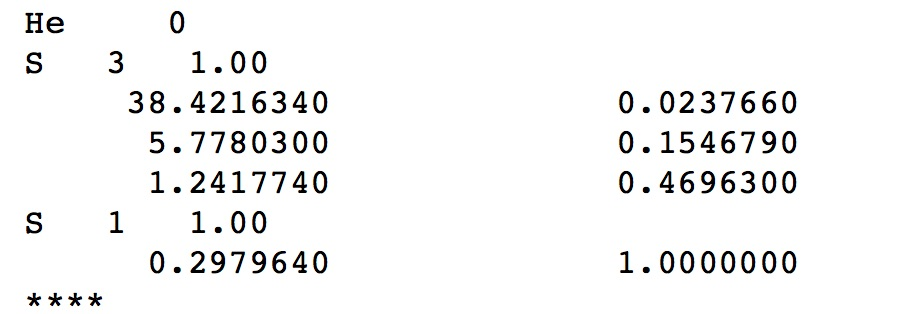
\includegraphics[height=0.8in]{figures/gaussian-he2.jpg}
\vspace{3mm}
\visible<2->{
\item 1st function has 3 Gaussians
\scriptsize{
\begin{eqnarray*}
\phi_1 & = &  N_t ( 0.023766 * N_1 *e^{-38.421634 r^2} \\ 
& & + 0.154679  * N_2 * e^{-5.77803 r^2} \\
& & + 0.46963 * N_3 * e^{-1.241774 r^2} ) 
\end{eqnarray*}
}
}
\vspace{-4mm}
\visible<3->{
\item \small{2nd function has 1 Gaussian}
\scriptsize{
\begin{equation*}
\phi_2 = N_4 e^{-0.2927640 r^2} 
\end{equation*}
}
}
\end{itemize}
\end{column}
\begin{column}{0.5\textwidth}
\vspace{-3mm}
\visible<4->{
\begin{center}
%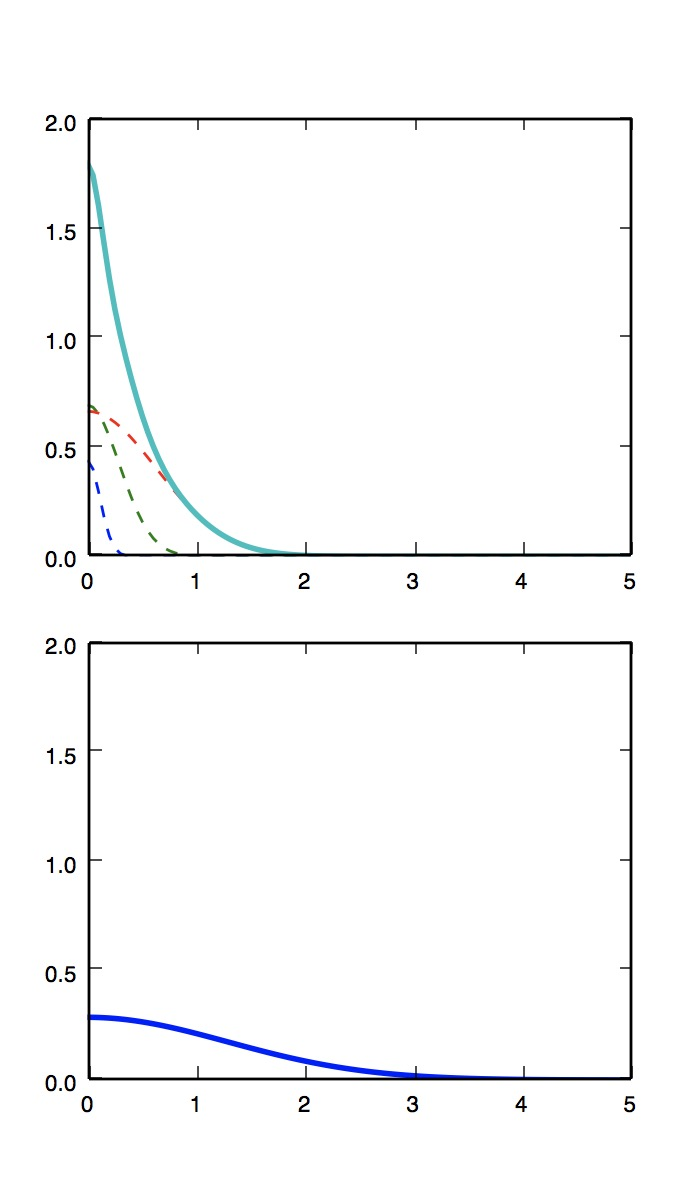
\includegraphics[height=3.2in]{figures/gaussian-he.jpg}
\end{center}
}
\end{column}
\end{columns}
\end{frame}

\begin{frame}
\frametitle{Pople Gaussian Basis Sets}
\scriptsize{
\begin{table}
\begin{tabular}{lcccc}
\hline \hline 
basis &  & H, He & Li, Be, B, C, N, O, F, Ne & Comment \\
\hline \\
STO-3G & core & &  3s $\rightarrow$ 1s & Too small   \\
    & valence & 3s $\rightarrow$ 1s & 3s3p $\rightarrow$ 1s1p &   \\  \\
\textcolor{red}{6}-\textcolor{blue}{31}G\textcolor{purple}{*} & core &  &   \textcolor{red}{6s  $\rightarrow$ 1s } & \\  
  & valence & \textcolor{blue}{4s  $\rightarrow$ 2s} & \textcolor{blue}{4s4p}\textcolor{purple}{1d}  $\rightarrow$ \textcolor{blue}{2s2p}\textcolor{purple}{1d} & \\  \\
\textcolor{red}{6}-31++G\textcolor{purple}{*}\textcolor{green}{*} & core & & \textcolor{red}{6s  $\rightarrow$ 1s} &  medium \\  
  & valence & 5s\textcolor{green}{1p}  $\rightarrow$ 3s\textcolor{green}{1p} & 5s5p\textcolor{purple}{1d}  $\rightarrow$ 3s3p\textcolor{purple}{1d} \\ \\
\textcolor{red}{6}-311++G\textcolor{purple}{*}\textcolor{green}{*} & core & & \textcolor{red}{6s  $\rightarrow$ 1s} &  large \\  
  & valence & 6s\textcolor{green}{1p}  $\rightarrow$ 4s\textcolor{green}{1p} & 6s6p\textcolor{purple}{1d}  $\rightarrow$ 4s4p\textcolor{purple}{1d} \\  \\
  \textcolor{red}{6}-311++G(3df,3pd) & core & & \textcolor{red}{6s  $\rightarrow$ 1s} &  largest \\
  & valence & 6s3p1d  $\rightarrow$ 4s3p1d & 6s6p3d1f $\rightarrow$ 4s4p3d1f \\ \\

\hline \hline
\end{tabular}
\end{table}
}
\begin{itemize}
\item See https://bse.pnl.gov/bse/portal for details
\visible<2->{
\item Dunning basis set (cc-pVDZ, aug-cc-pVDZ, cc-pVTZ, aug-cc-pVTZ, cc-pVQZ, aug-cc-pVQZ) are equally (if not more) popular}
\end{itemize}

\end{frame}


\begin{frame}
\frametitle{Hartree-Fock Solutions for the Helium Atom}

\begin{itemize}
\item With exponential functions, the lowest energy was -2.861680
\item 6-31G, Energy is -2.855160 
\item 6-31G**, Energy is -2.855160
\item 6-31++G**, Energy is -2.855720
\item 6-311G, Energy is -2.859895
\item 6-311++G**, Energy is -2.860006
\item aug-cc-pVQZ, Energy is -2.861522
\end{itemize}

\end{frame}


\section{Homework}

\begin{frame}
\begin{itemize}
\item 2 Points. Due at 8am, Monday, October 31.

\vspace{4mm}
\visible<2->{
\item \textcolor{blue}{Homework 8.1.}   Compute the Hartree-Fock energy of the hydrogen atom 
\begin{itemize}
\item Use IQmol (iqmol.org), or WebMO (webmo.net), or Spartan
\item Use at least three basis sets, such as 6-31G*, 6-31+G*, 6-311G**, 6-311++G**, aug-cc-pVDZ, aug-cc-pVTZ, and aug-cc-pVQZ.   
\end{itemize}
}

\vspace{4mm}
\visible<3->{
\item \textcolor{blue}{Homework 8.2.}    Compute the Hartree-Fock energy for the \textcolor{red}{triplet} state of the helium atom
\begin{itemize}
\item Use IQmol, WebMO or Spartan
\item Use at least three basis sets
\end{itemize}
}

\end{itemize}

\end{frame}

\end{document}

\begin{frame}
\frametitle{Blank Page}
\begin{columns}
\begin{column}{0.4\textwidth}
\begin{center}
\end{center}
\end{column}
\begin{column}{0.6\textwidth}
\begin{center}
\end{center}
\end{column}
\end{columns}
\end{frame}

